\chapter{Resultate}
\label{ch_resultat}

Im Kapitel \ref{ch_vorgehen} ist die Umsetzung ausführlich erklärt. In diesem Kapitel geht es um die relevanten Resultate. Diese teilen sich in die bekannten Kategorien Harvester, Energy und Power Management sowie die BLE-Applikation. Die Resultate jeder Kategorie werden in einem Unterkapitel beschrieben.
 
\section{Harvesterschaltung}

\subsection{Der Print}

Das erste konkrete Resultat ist der fertige Print. In der Abbildung \ref{print_vorne} ist die Vorderseite abgebildet. \todo{bessere Beschreibung} Darauf befindet sich im Wesentlichen der Header als Verbindungsstecker zum Sensortag, die vier Gleichrichterdioden, der Limiter, die Spule und der EM8500. In der Abbildung \ref{print_rueckseite} befindet sich der Reed-Switch und die dreilagige Premo-Spule, mit der die Induktion erzeugt wird.

\begin{figure}[ht]
    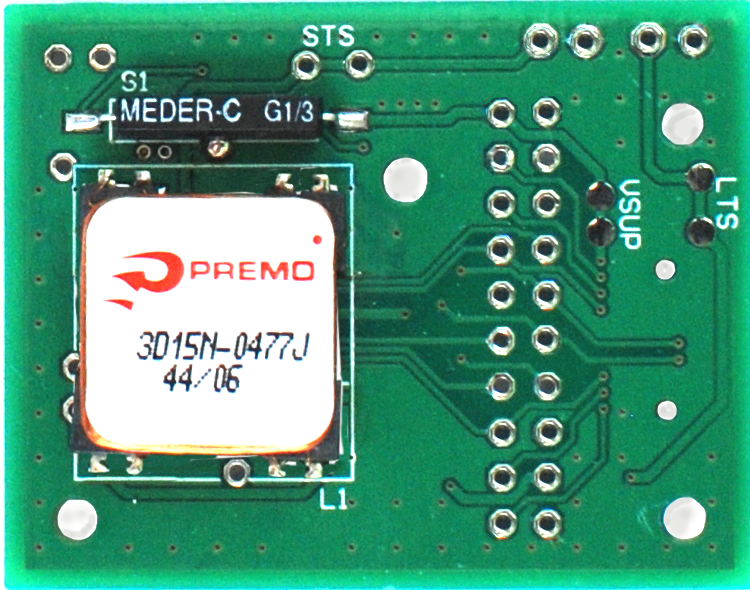
\includegraphics[width=0.5\textwidth]{4Resultate/imag/print_rueckseite.png} 
    \caption{Print Vorderseite}
    \label{print_vorne}
\end{figure}


\begin{figure}[ht]
    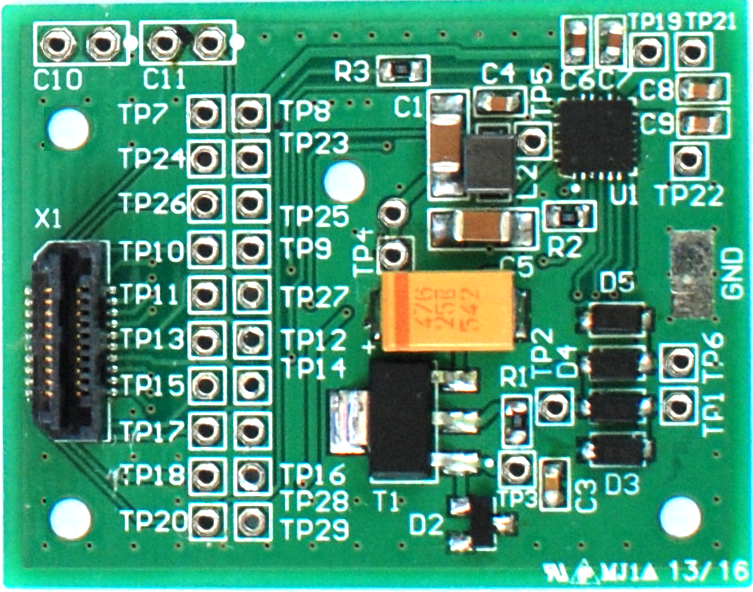
\includegraphics[width=0.5\textwidth]{4Resultate/imag/print_vorne.png} 
    \caption{Print Rückseite}
    \label{print_rueckseite}
\end{figure}

\newpage  % todel
\subsection{Leistung am Harvesterausgang}

Wie erwartet (siehe theoretische Grundlagen \ref{mpp_theorie_diff}) ändert sich bei einer Hardware mit Spule das Leistungsmaximum. Die Abbildung \ref{mpp_resultat_harvester} zeigt die reale MPP-Kurve des Prototypen. Bei 10 km/h liegt das Leistungsmaximum bei \todo{xxx mW}, bei 15 km/h bei \todo{xxx mW}, bei 20 km/h bei\todo{xxx mW} und bei 40 km/h bei \todo{xxx mW}. Die detaillierten Angaben finden sich im Messprotokoll \todo{Name Messprotokoll}

\begin{figure}[ht]
    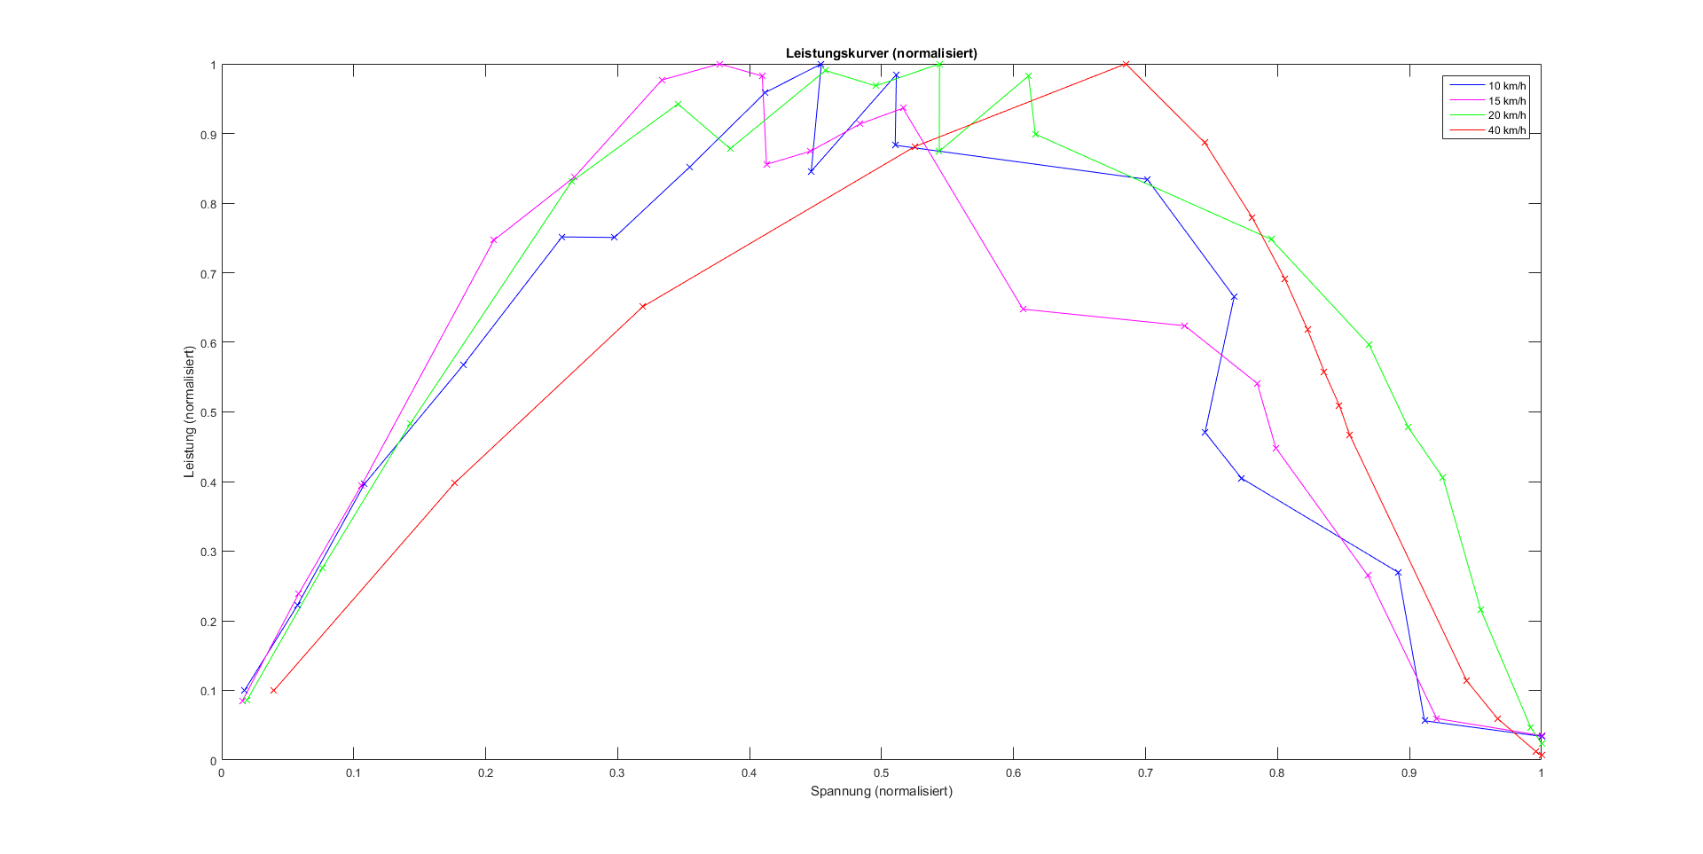
\includegraphics[width=0.5\textwidth]{4Resultate/imag/MPPHarvester.png} 
    \caption{Leistungskurve Harvesterausgang (normalisiert)}
    \label{resultat_Harvester_Spannung}
\end{figure}


\newpage  % todel
\subsection{Verhalten des Harvesterausgangs}

Die Abbildung \ref{resultat_Harvester_Spannung} zeigt, das reelle Verhalten des Harvesters bei Belastung mit dem EM-Chip. Wie in beschrieben \ref{optimaleLeistung} regelt der Chip EM8500 den Eingang, bzw. den Ausgang des Harvesters, um den MPP zu erreichen. Die Abbildung \ref{resultat_Harvester_Spannung} zeigt den Verlauf der geregelten Spannung am Eingang des EM-Chips über längere Zeit. Weitere Messungen zum reelen Verhalten am EM8500-Chip-Eingang können den Messprotokoll \todo{Namen heraussuchen} entnommen werden.

\begin{figure}[ht]
    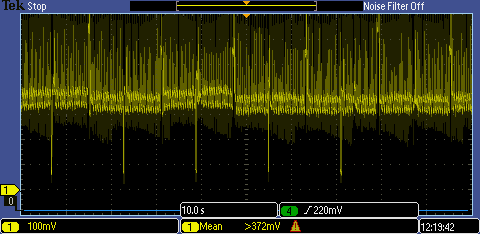
\includegraphics[width=0.5\textwidth]{4Resultate/imag/SpannungVCC.png} 
    \caption{Spannung VCC beim Harvesterausgang bei 15 km/h}
    \label{resutat_emchip_spannung}
\end{figure}

\newpage  % todel
\subsection{Energie am EM-Chipausgang}

Die Energie, welche vom EM-Chip abgegeben wird, steigt mit der Geschwindigkeit. Hier wurde die Energie von einem Puls gemessen, d.h. vom Einschalten von VSUP bis zur Abschaltung von VSUP. Nach diesem Puls wird keine Energie mehr abgegeben, bis zum nächsten Puls.


\begin{figure}[ht]
    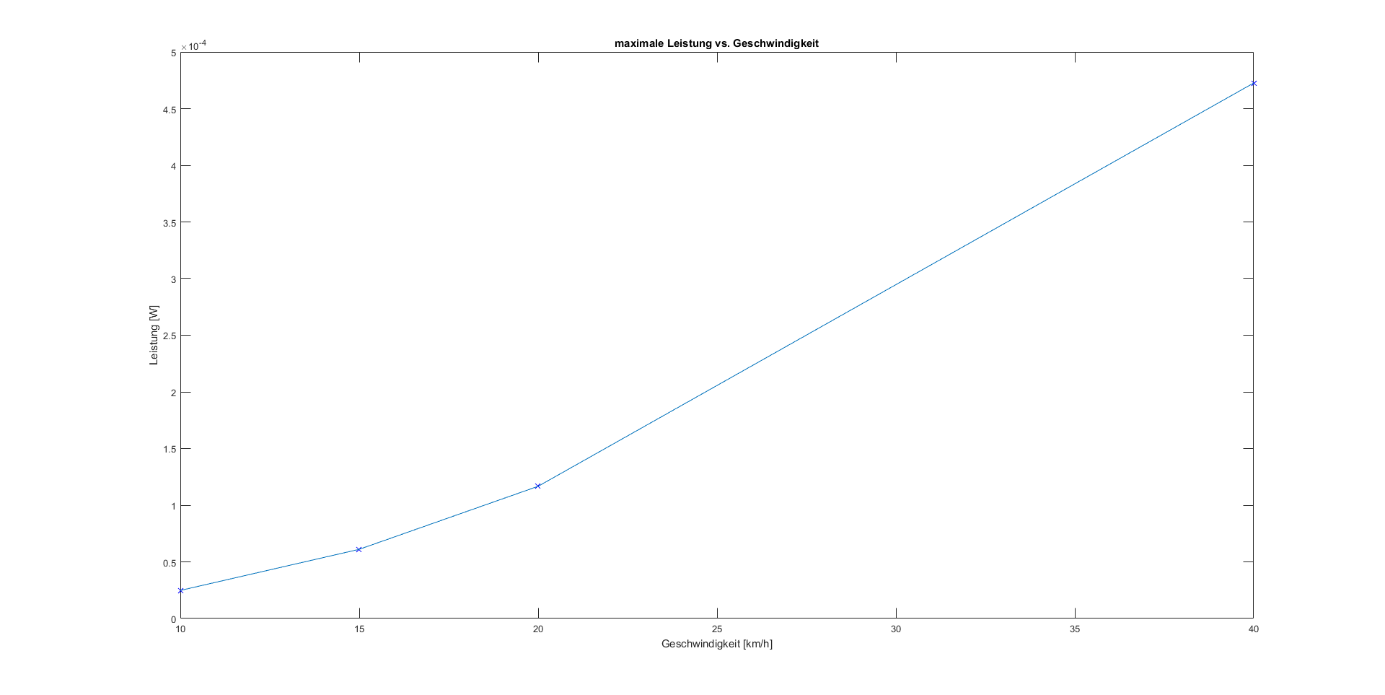
\includegraphics[width=0.5\textwidth]{4Resultate/imag/ResultatLeistungGeschwindigkeit.png} 
    \caption{Maximale Leistung vs. Geschwindigkeit}
    \label{mpp_resultat_harvester}
\end{figure}

\subsection{Wirkungsgrad des Prototypen}

Interessant ist die Betrachtung des Wirkungsgrades des EM-Chips. In der nachfolgenden Tabelle sind die Leistungen aufgezeichnet, welche mit den aktuellen Einstellungen des EM-Chips anliegen.

\subsubsection*{Tabelle Leistung und Wirkungsgrad }
\begin{tabbing}
    Geschwindigkeit \quad\= Leistung Harvester \quad\= Leistung EM8500\_out \quad\= Wirkungsgrad\\[0.8ex]
    10 km/h  \> 21.87  $\mu$W \> 5.44   $\mu$W \> 24.87\thinspace\%  \\
    15 km/h  \> 57.19  $\mu$W \> 20.91  $\mu$W \> 36.56\thinspace\%  \\
    20 km/h> \> 114.67 $\mu$W \> 41.39  $\mu$W \> 36.09\thinspace\%  \\
    40 km/h> \> 416.29 $\mu$W \> 170.75 $\mu$W \> 41.01\thinspace\%  \\
\end{tabbing}   

Die Abbildung \ref{zsmEnergyGewinn} gibt einen Überblick, an welcher Stelle wie viel Energie vorhanden ist, bzw. zwischen welchen zwei Stellen wie viel Energie verloren ging.

\begin{figure}[ht]
    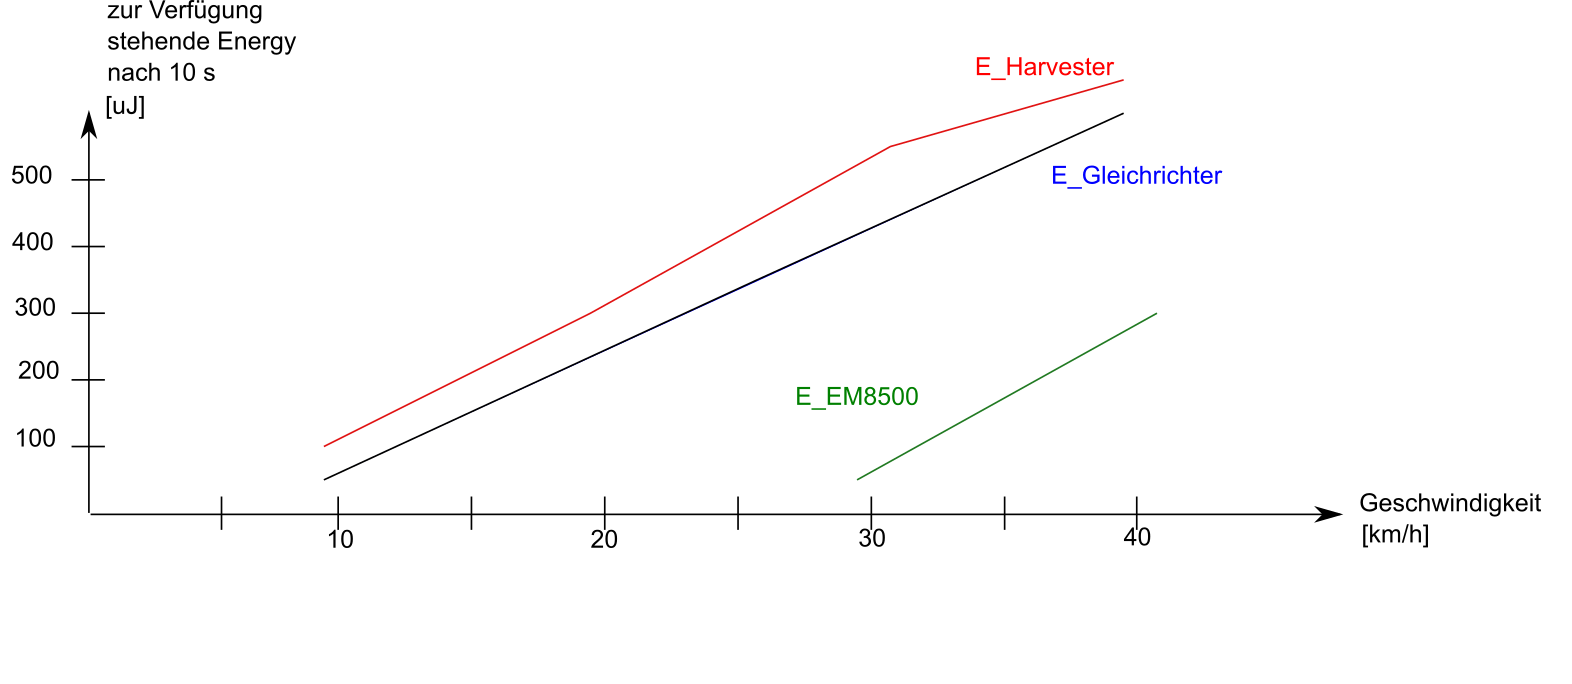
\includegraphics[width=1\textwidth]{4Resultate/imag/EnergyGewinnNachStelle.png} 
    \caption{Energiegewinn Zusammengefasst nach Stelle in der Schaltung}
    \label{zsmEnergyGewinn}
\end{figure}

Der Wirkungsgrad des EM8500 innerhalb des entwickelten Prototypen liegt bei 40 km/h  bei 41.01\thinspace\% und bei 10 km/h bei 24.87\thinspace\%.


\section{Energiemanagement}

%Beim Resultat spielt das Hard- und Softwaremanagment direkt ineinander, weshalb das Ergebnisse dieser zwei Aufgaben zusammen dargestellt werden.

Durch das korrekte Einstellen der Schwellwerte beim EM8500 (siehe Unterkapitel xxx) und die korrekten Ladewerte bei den Kondensatoren (siehe Unterkaptiel xxx), ist es möglich, dass sich der LTS-Kondensator bei einer Geschwindigkeit von YYY km/h lädt (siehe Abbildung xxx). Zudem entlädt sich LTS, sobald das Sensortag am Arbeiten ist (siehe Abbildung yyyy). Beim Energiemanagement ist es somit gelungen, die Schwellwerte und Kondensatorengrössen so einzustellen, dass die Funktionalitäten des EM8500-Chips voll ausgenutzt werden können.

\begin{figure}[ht]
    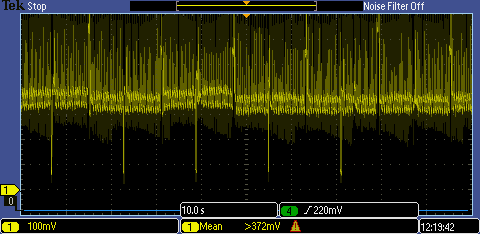
\includegraphics[width=0.1\textwidth]{4Resultate/imag/SpannungVCC.png} 
    \caption{STS und LTS laden sich}
\end{figure}

\begin{figure}[ht]
    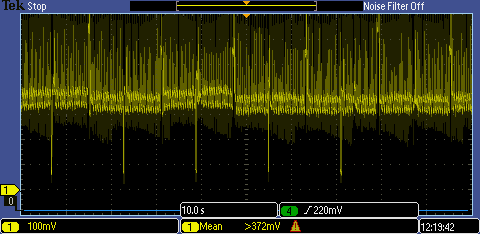
\includegraphics[width=0.1\textwidth]{4Resultate/imag/SpannungVCC.png} 
    \caption{LTS liefert Energie für die Arbeitspakete}
\end{figure}


\section{Powermanagement}

Durch ein gutes Powermanagement (siehe Unterkapitel xxx) wurde es möglich, die energiestarken Aufgaben in Teilen zu erledigen. Die Abbildung xxxx zeigt, das Aufteilen der Arbeitsschritte: Zuerst folgt das Init, dann folgt das Auslesen eines Sensors, dann das Senden des Sensors. Die Aufgaben wurden aufgeteilt, weil alle drei Schritte in einem zu viel Energie verbraucht hätte, sodass VSUP zusammengebrochen wäre.

\begin{figure}[ht]
    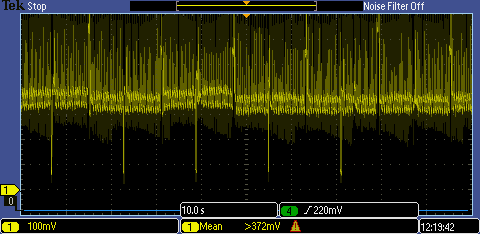
\includegraphics[width=0.1\textwidth]{4Resultate/imag/SpannungVCC.png} 
    \caption{Drei Arbeitspakte bis zum Senden der Daten }
    \label{blub}
\end{figure}

\todo{ ev. Grossaufnahme: BLE Energieverbrauch}

Die Abbildung \ref{resultat_E_Verbrauch_Verarbeitungsaufwand} zeigt den Energieverbrauch nach Verarbeitungsaufwand. Am wenigsten Energie benötigt das Berechnen der Geschwindigkeit über den RTC. Deutlich mehr Energie braucht das Auslesen der Sensor-Daten. Dies einerseits, weil die I2C-Kommunikation aufgebaut werden muss und weil die Sensoren eine gewisse Zeit brauchen, bis sie aktiv sind \todo{Aufwachzeit eines Sensors messen}. Die unterschiedlich verbrauchten Energiemengen entsprechen exakt den unterschiedlichen Startzeiten der Sensoren. 

\begin{figure}[ht]
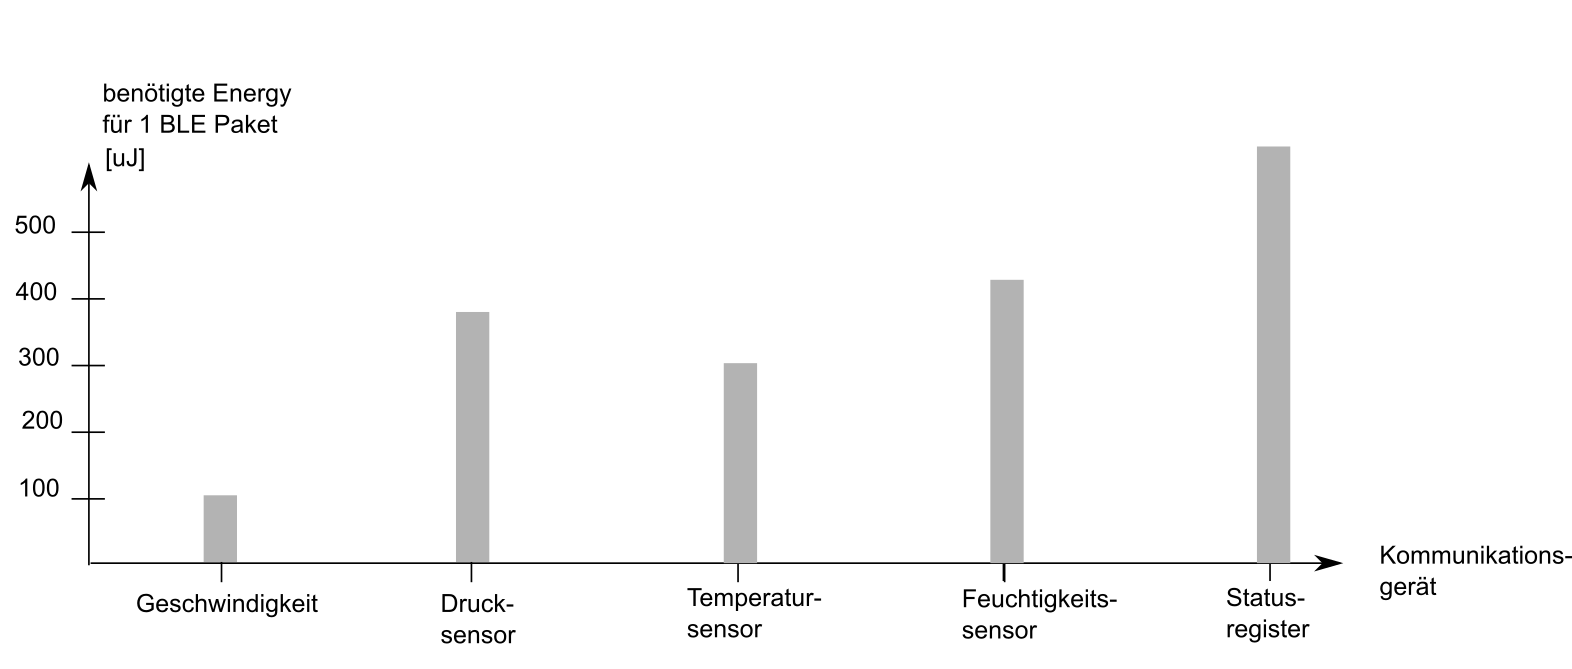
\includegraphics[width=1\textwidth]{4Resultate/imag/EnergyVerbrauchNachKommunikation.png} \label{resultat_E_Verbrauch_Verarbeitungsaufwand} 
\caption{Energieverbrauch gemäss Verarbeitungsaufwand für CPU}
\end{figure}

Kombiniert man den Energieverbrauch mit der zur Verfügung stehenden Energie am Ausgang nach dem EM8500-Chips, können (siehe Abbildung \ref{resultat_Zsm_Energy}) folgende Schlussfolgerungen gezogen werden:

\begin{enumerate}
    \item bla
    \item bla
    \item bla
    \item bla
\end{enumerate}

\begin{figure}[ht]
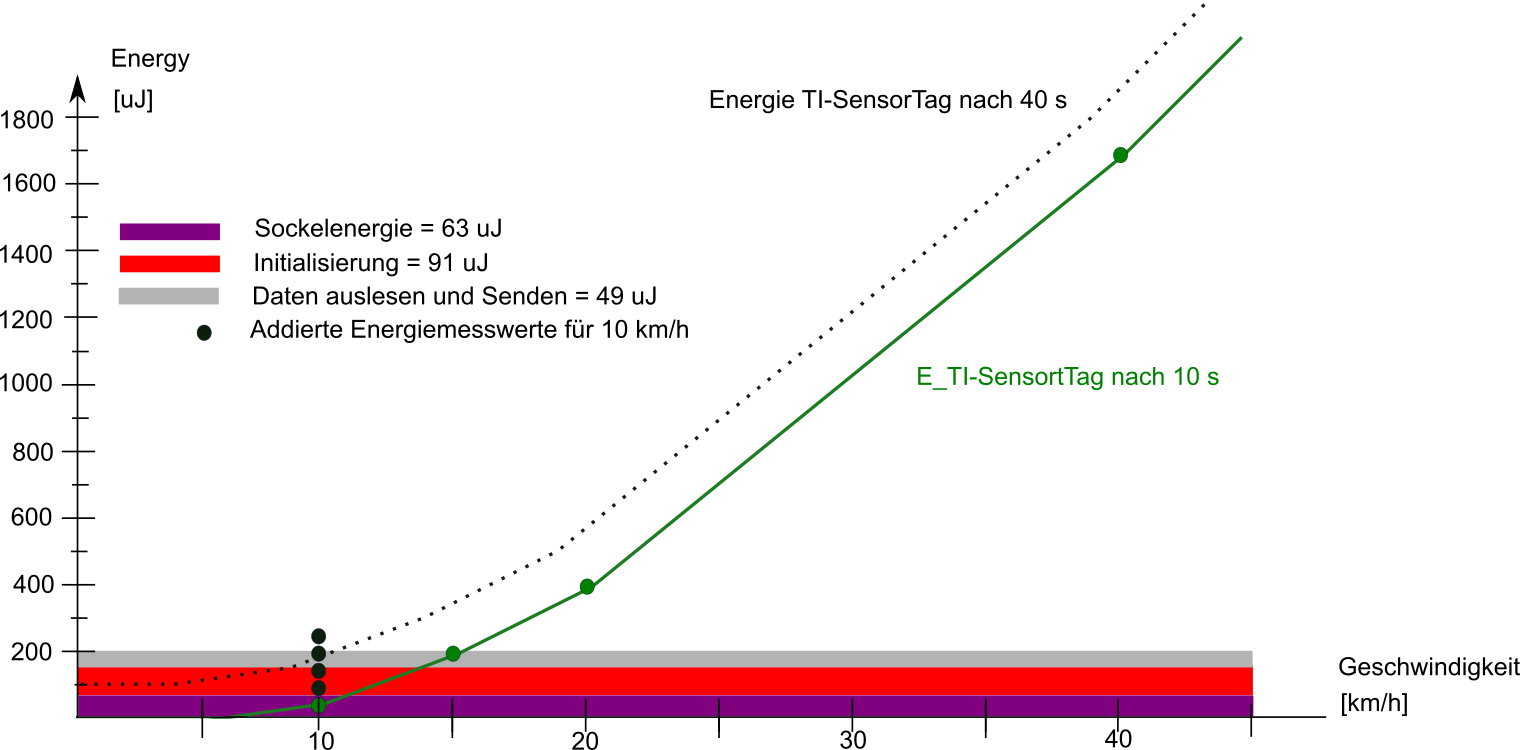
\includegraphics[width=1\textwidth]{4Resultate/imag/EnergyVerbrauchZusammenfassung.png}\label{resultat_Zsm_Energy} 
\caption{Energieverbrauch gem\"{a}ss Verarbeitungsaufwand für CPU}
\end{figure}


\section{Ergebnisse BLE-Applikation}

Der Aufbau des Sensortags zusammen mit dem selbst entwickelten Board wird \glqq Sensor\grqq\thinspace\ genannt. Dies, weil aus der Sicht einer Benutzerin oder eines Benutzers keine detaillierte Hardware besteht, sondern \glqq ein Sensor\grqq. Die Vereinfachung dient der Benutzerfreundlichkeit. Die Android-Applikation ist bewusst einfach aufgebaut, um die Benutzerin bzw. den Benutzer nicht zu verwirren. 

Der animierte Tachometer stellt die aktuelle Geschwindigkeit schnell und übersichtlich dar. Weitergehende Funktionen sind durch prägnante Namen selbsterklärend und der User sollte keine Mühe haben, die App ohne Lesen einer Anleitung zu verstehen.

\subsection{Applikationsstruktur}

Beim Öffnen der Applikation wird geprüft, ob Bluetooth aktiviert ist (siehe Abbildung \ref{permission}). Sollte Bluetooth nicht aktiviert sein, wird der User gefragt, ob Bluetooth aktiviert werden darf. Sollte der User die Aktivierung ablehnen schliesst sich die Applikation sofort.

\begin{figure}[ht]
    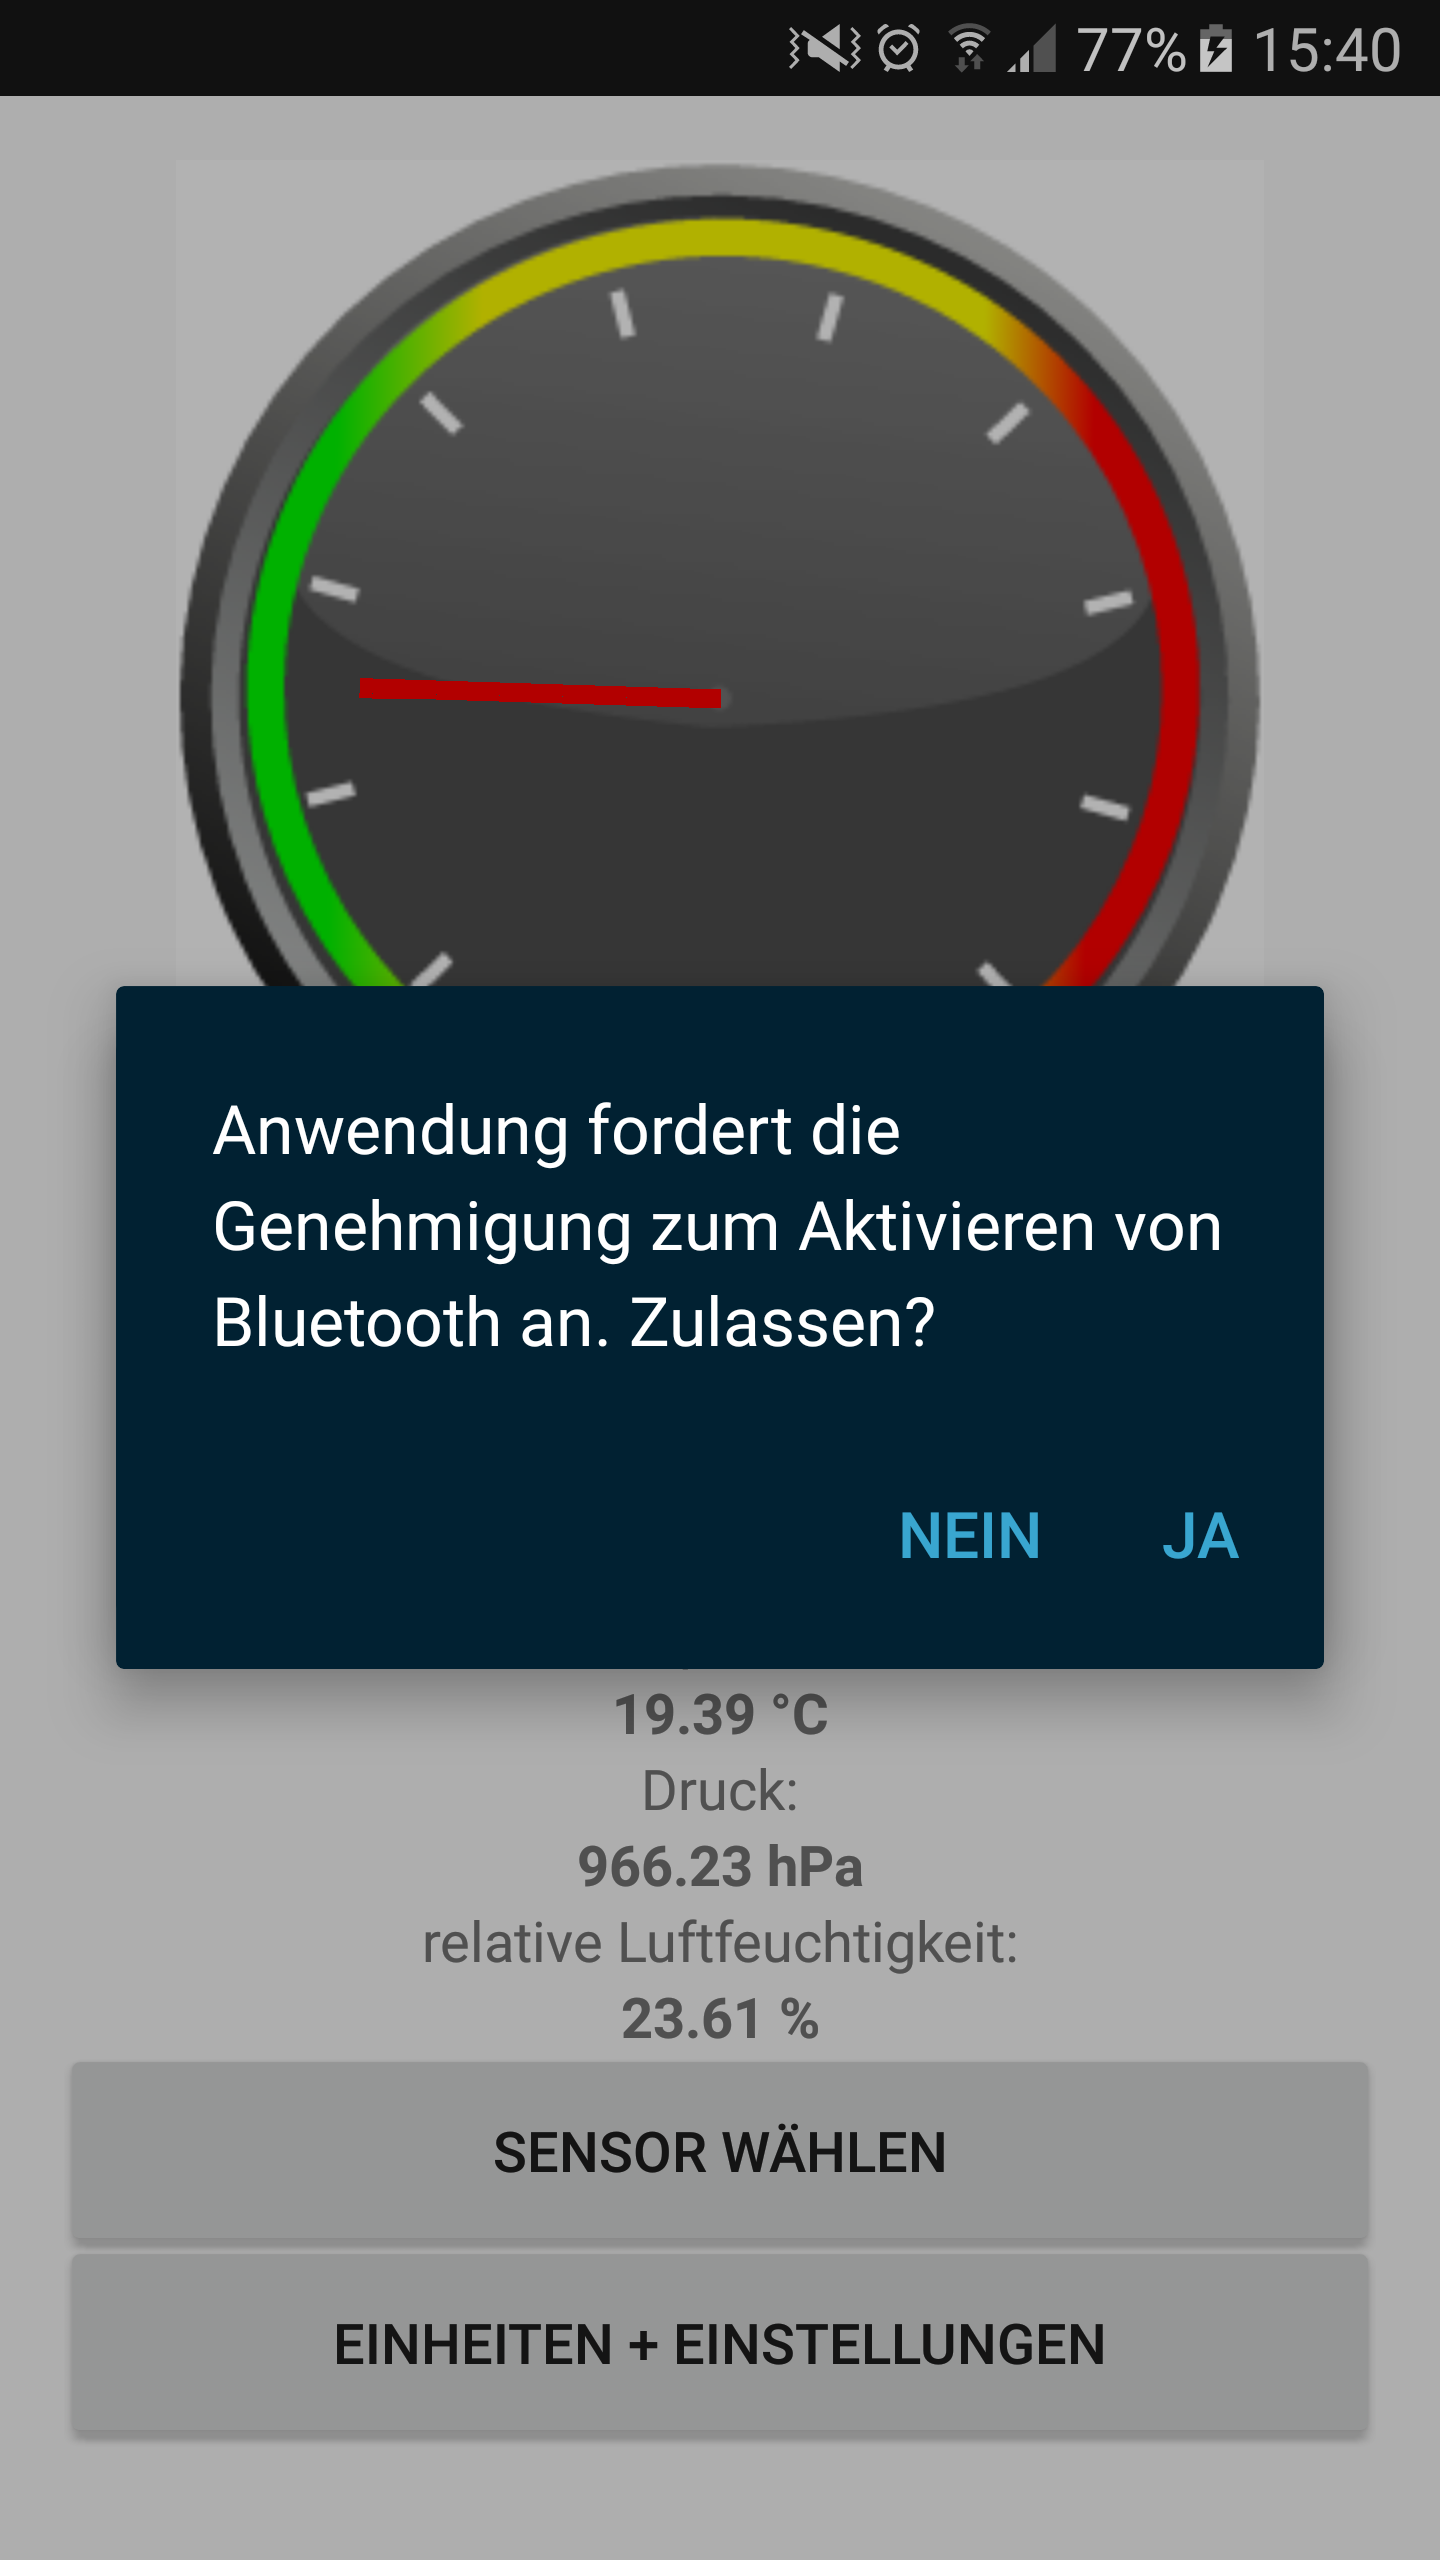
\includegraphics[width=0.5\textwidth]{4Resultate/imag/BLEBluetoothPermission.png} 
    \caption{Bluetooth Permission}
    \label{permission}
\end{figure}

Wird eine Verbund zu Bluetooth erlaubt, erscheint der Startbildschirm. Auf diesem befindet sich zentral der Tachometer (siehe Abbildung \ref{tacho}). Dieser zeigt Geschwindigkeiten von 0 – 90 km/h mit einer animierten Tachonadel an. Unterhalb des Tachometers werden die einzelnen Sensordaten angezeigt und im untersten Teil des Startbildschirms befinden sich zwei Buttons, über die man Einstellungen vornehmen kann. Die Kontextmenus zu diesen Einstellungen werden in den nächsten zwei Abbildungen \ref{sensorauswahl} und \ref{einheiten} ersichtlich. 

\begin{figure}[ht]
    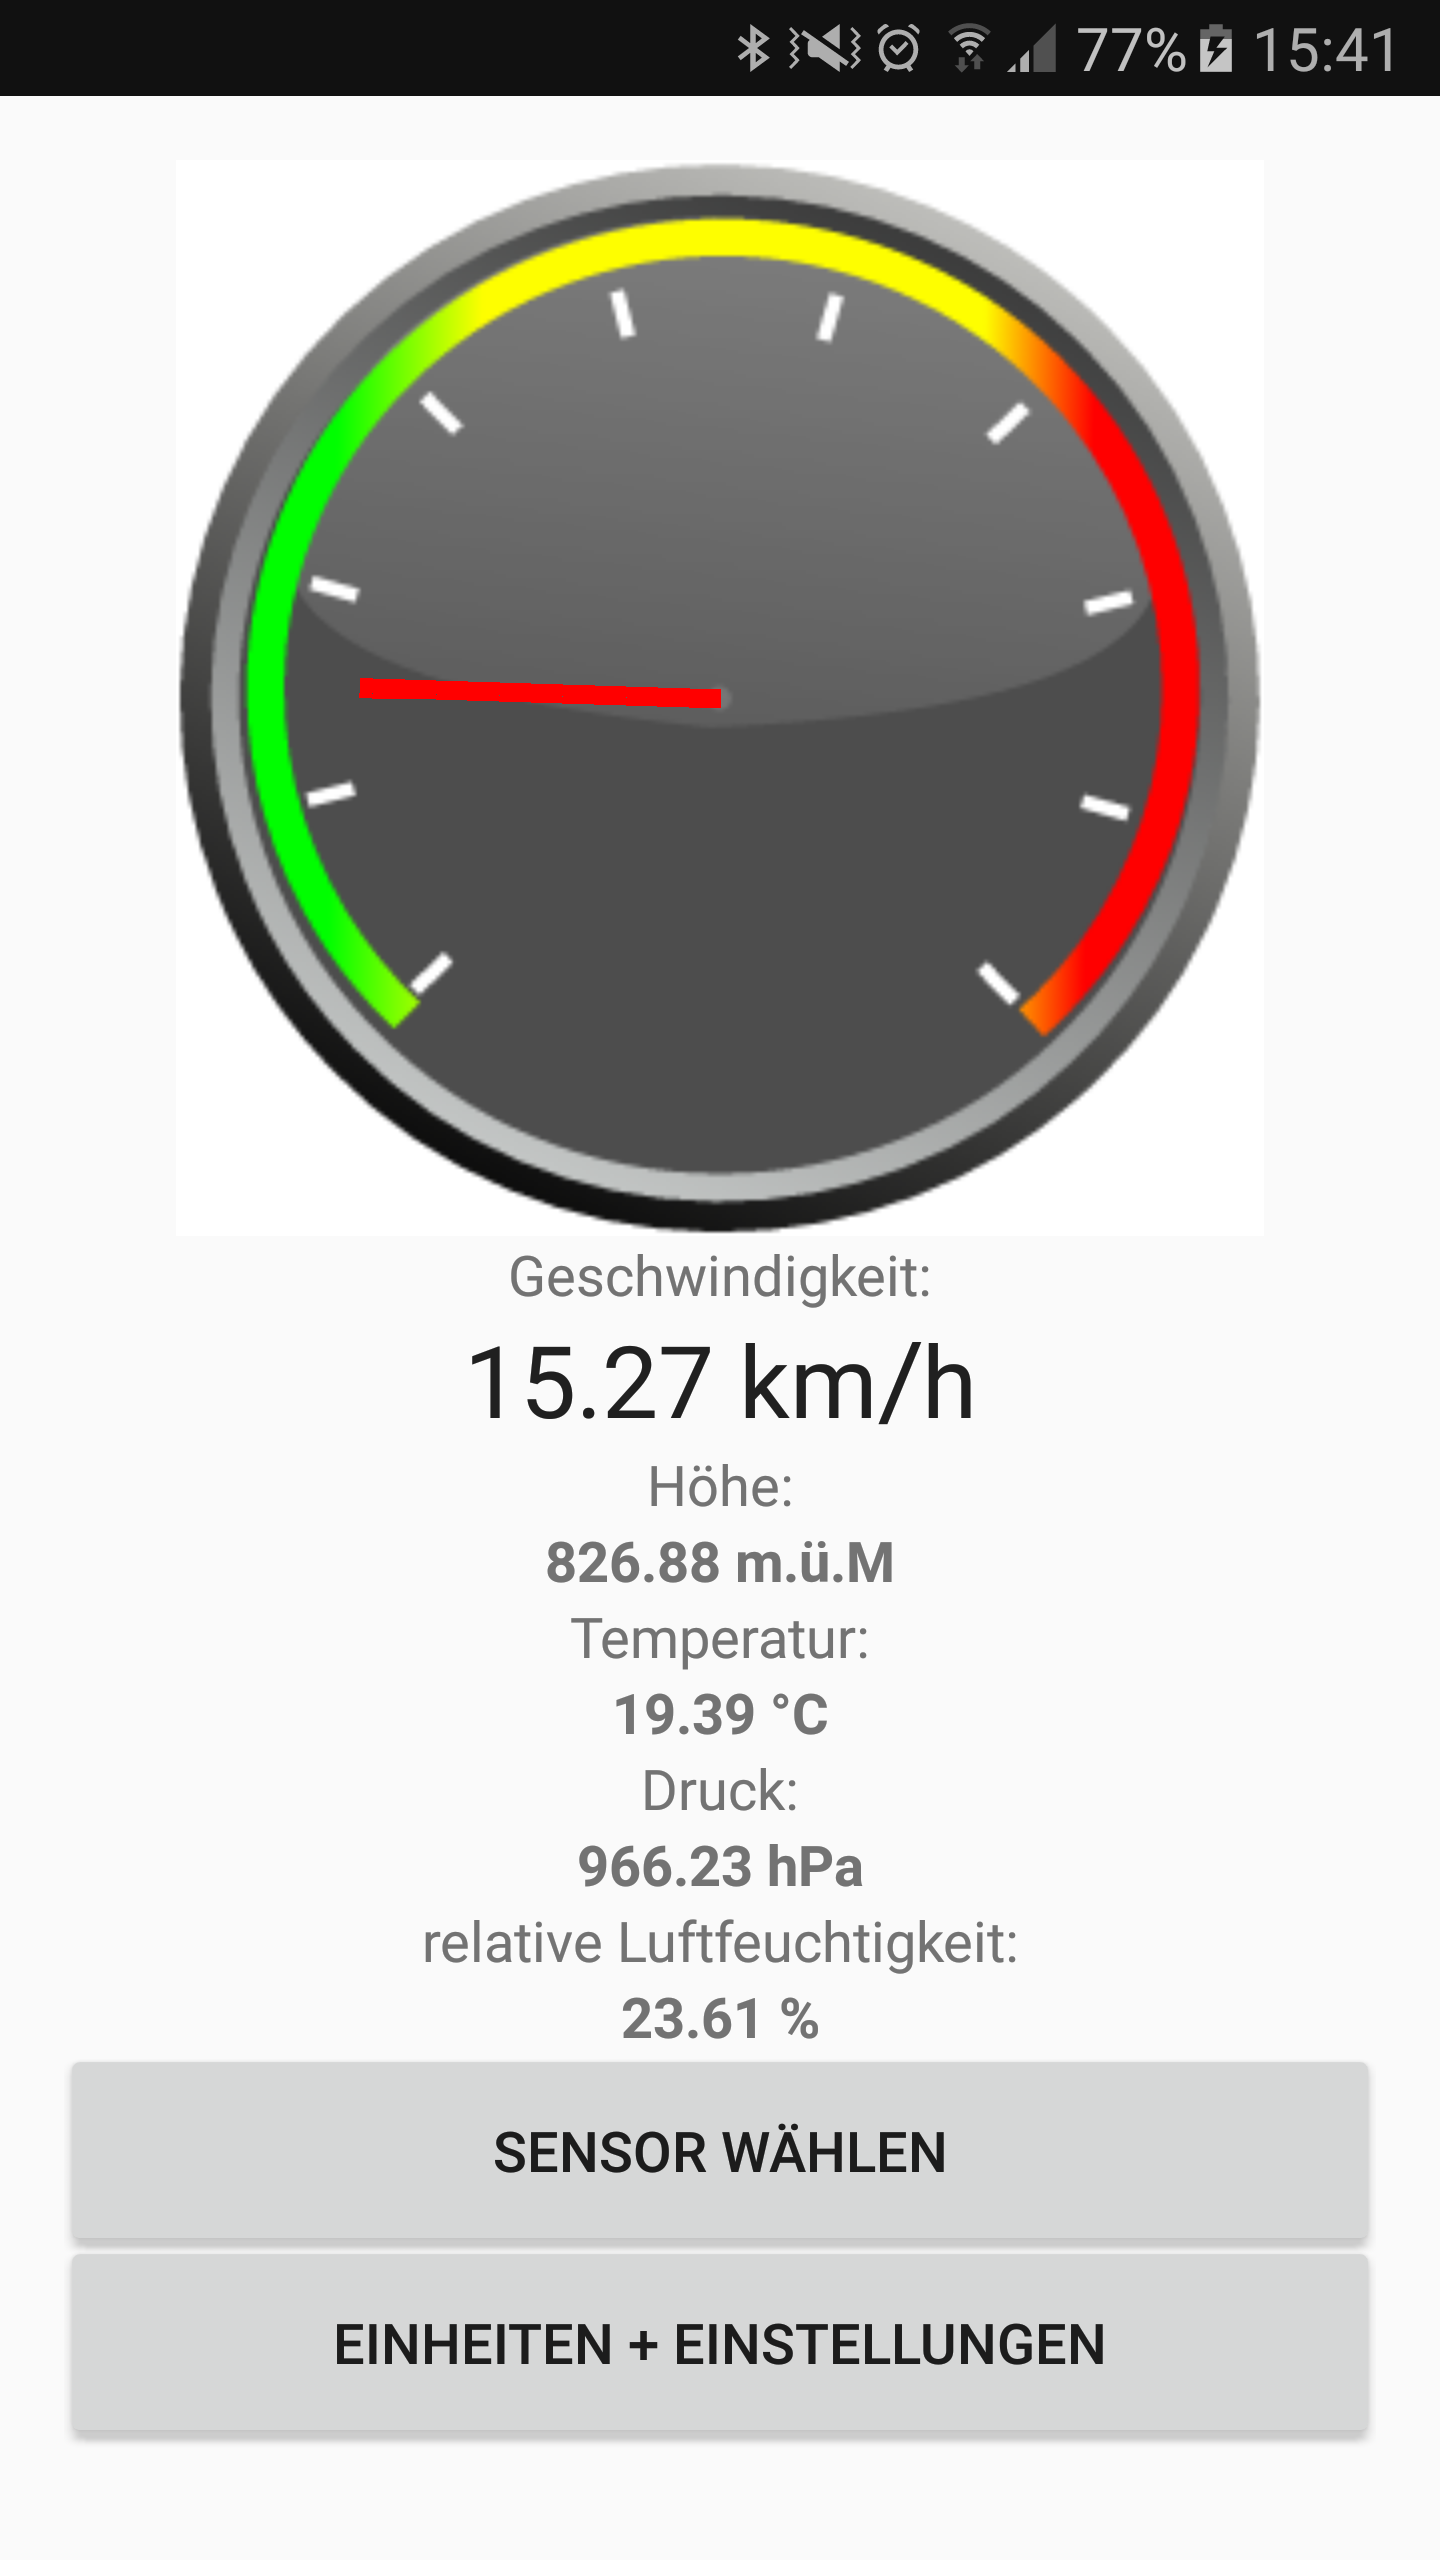
\includegraphics[width=0.5\textwidth]{4Resultate/imag/APPHomeScreen.png} 
    \caption{Startbildschirm der Applikation}
    \label{tacho}
\end{figure}

Wählt man auf dem Startbildschirm \glqq Sensor wählen\grqq, \todo{ev. besser: Sensorboard wählen} erscheint ein neuer Bildschirm. Auf diesem erscheinen nur die aktiven Bluetooth Geräte mit dem implementierten Prototypen-Filter. Der Bildschirm bildet die Sensortagadresse ab. \todo{Text: warum user das Sensor nennt. Und es dehalb so heisst und nicht Board}. Jedes Sensortag hat eine eigene Adresse und bei mehreren Prototypen im Raum, kann das entsprechende Gerät ausgewählt werden.


\begin{figure}[ht]
    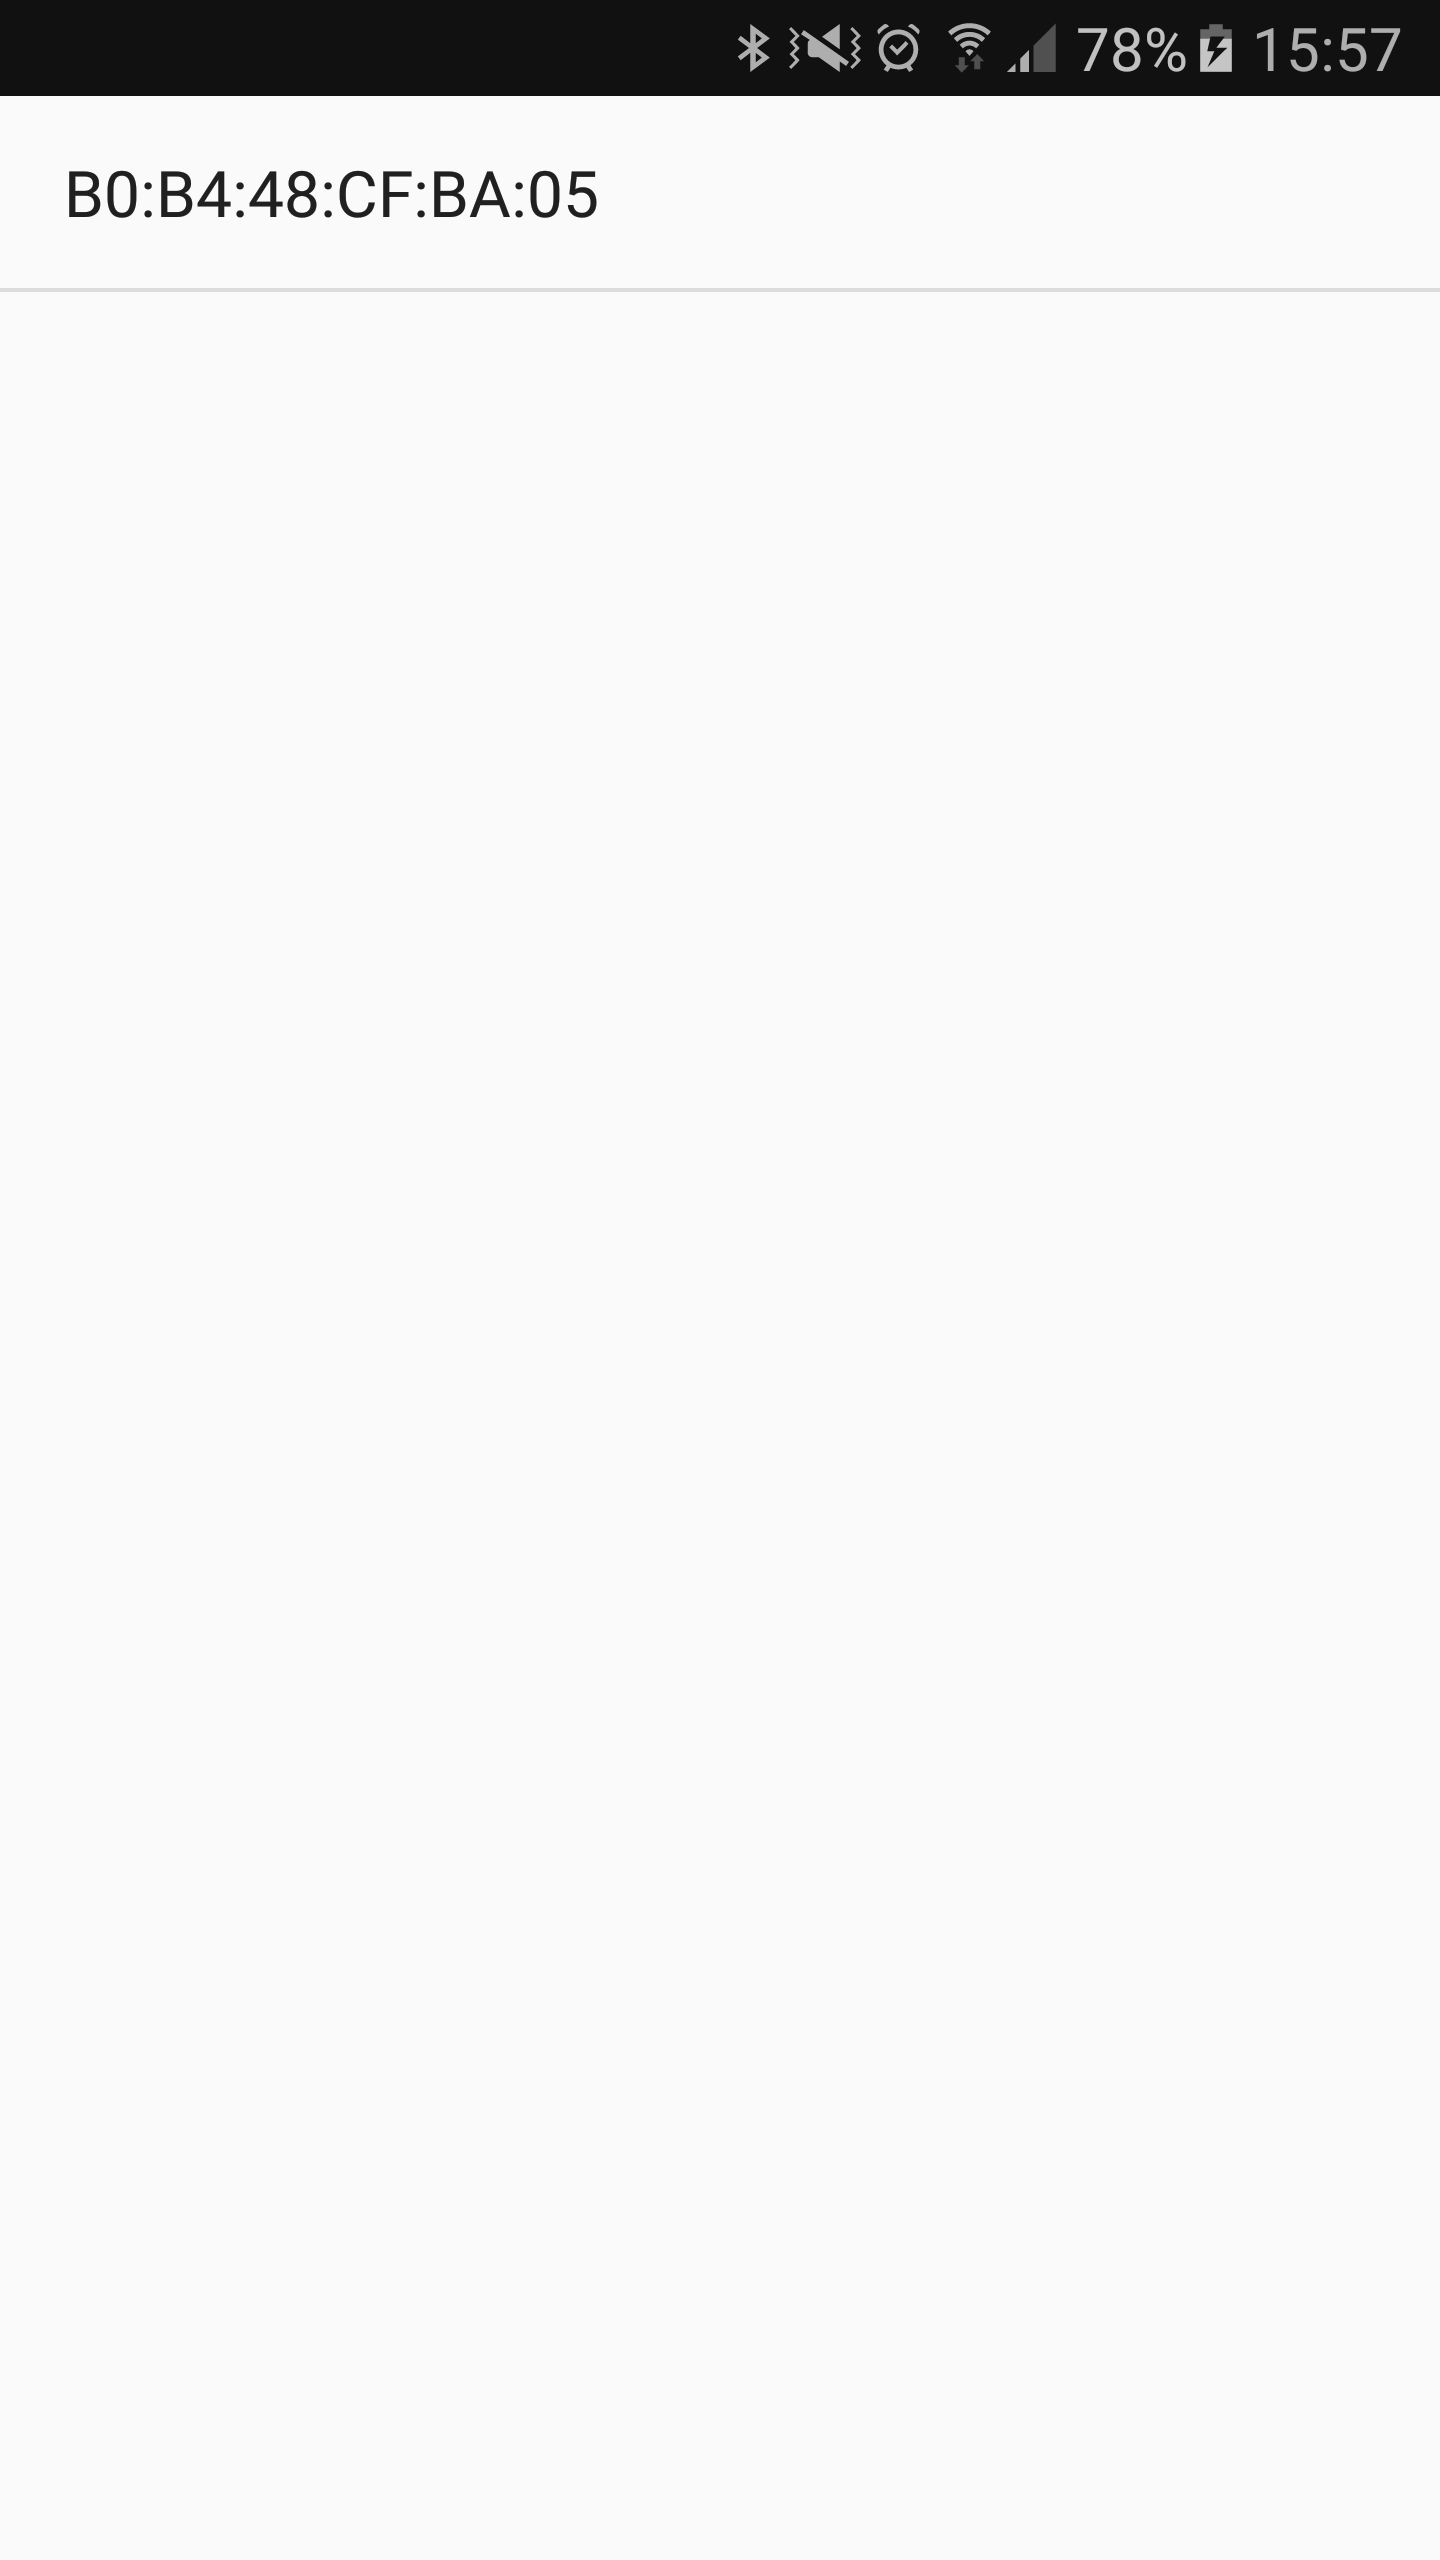
\includegraphics[width=0.5\textwidth]{4Resultate/imag/BLEAdresseAuswaehlen.png} 
    \caption{Sensortagauswahl}
    \label{sensorauswahl}
\end{figure}

Auf dem Startbildschirm befindet sich auch ein Konfigurationsknopf. In das Untermenu gelangt man, in dem man den Button "Einheiten + Einstellungen" auswählt.

\begin{figure}[ht]
    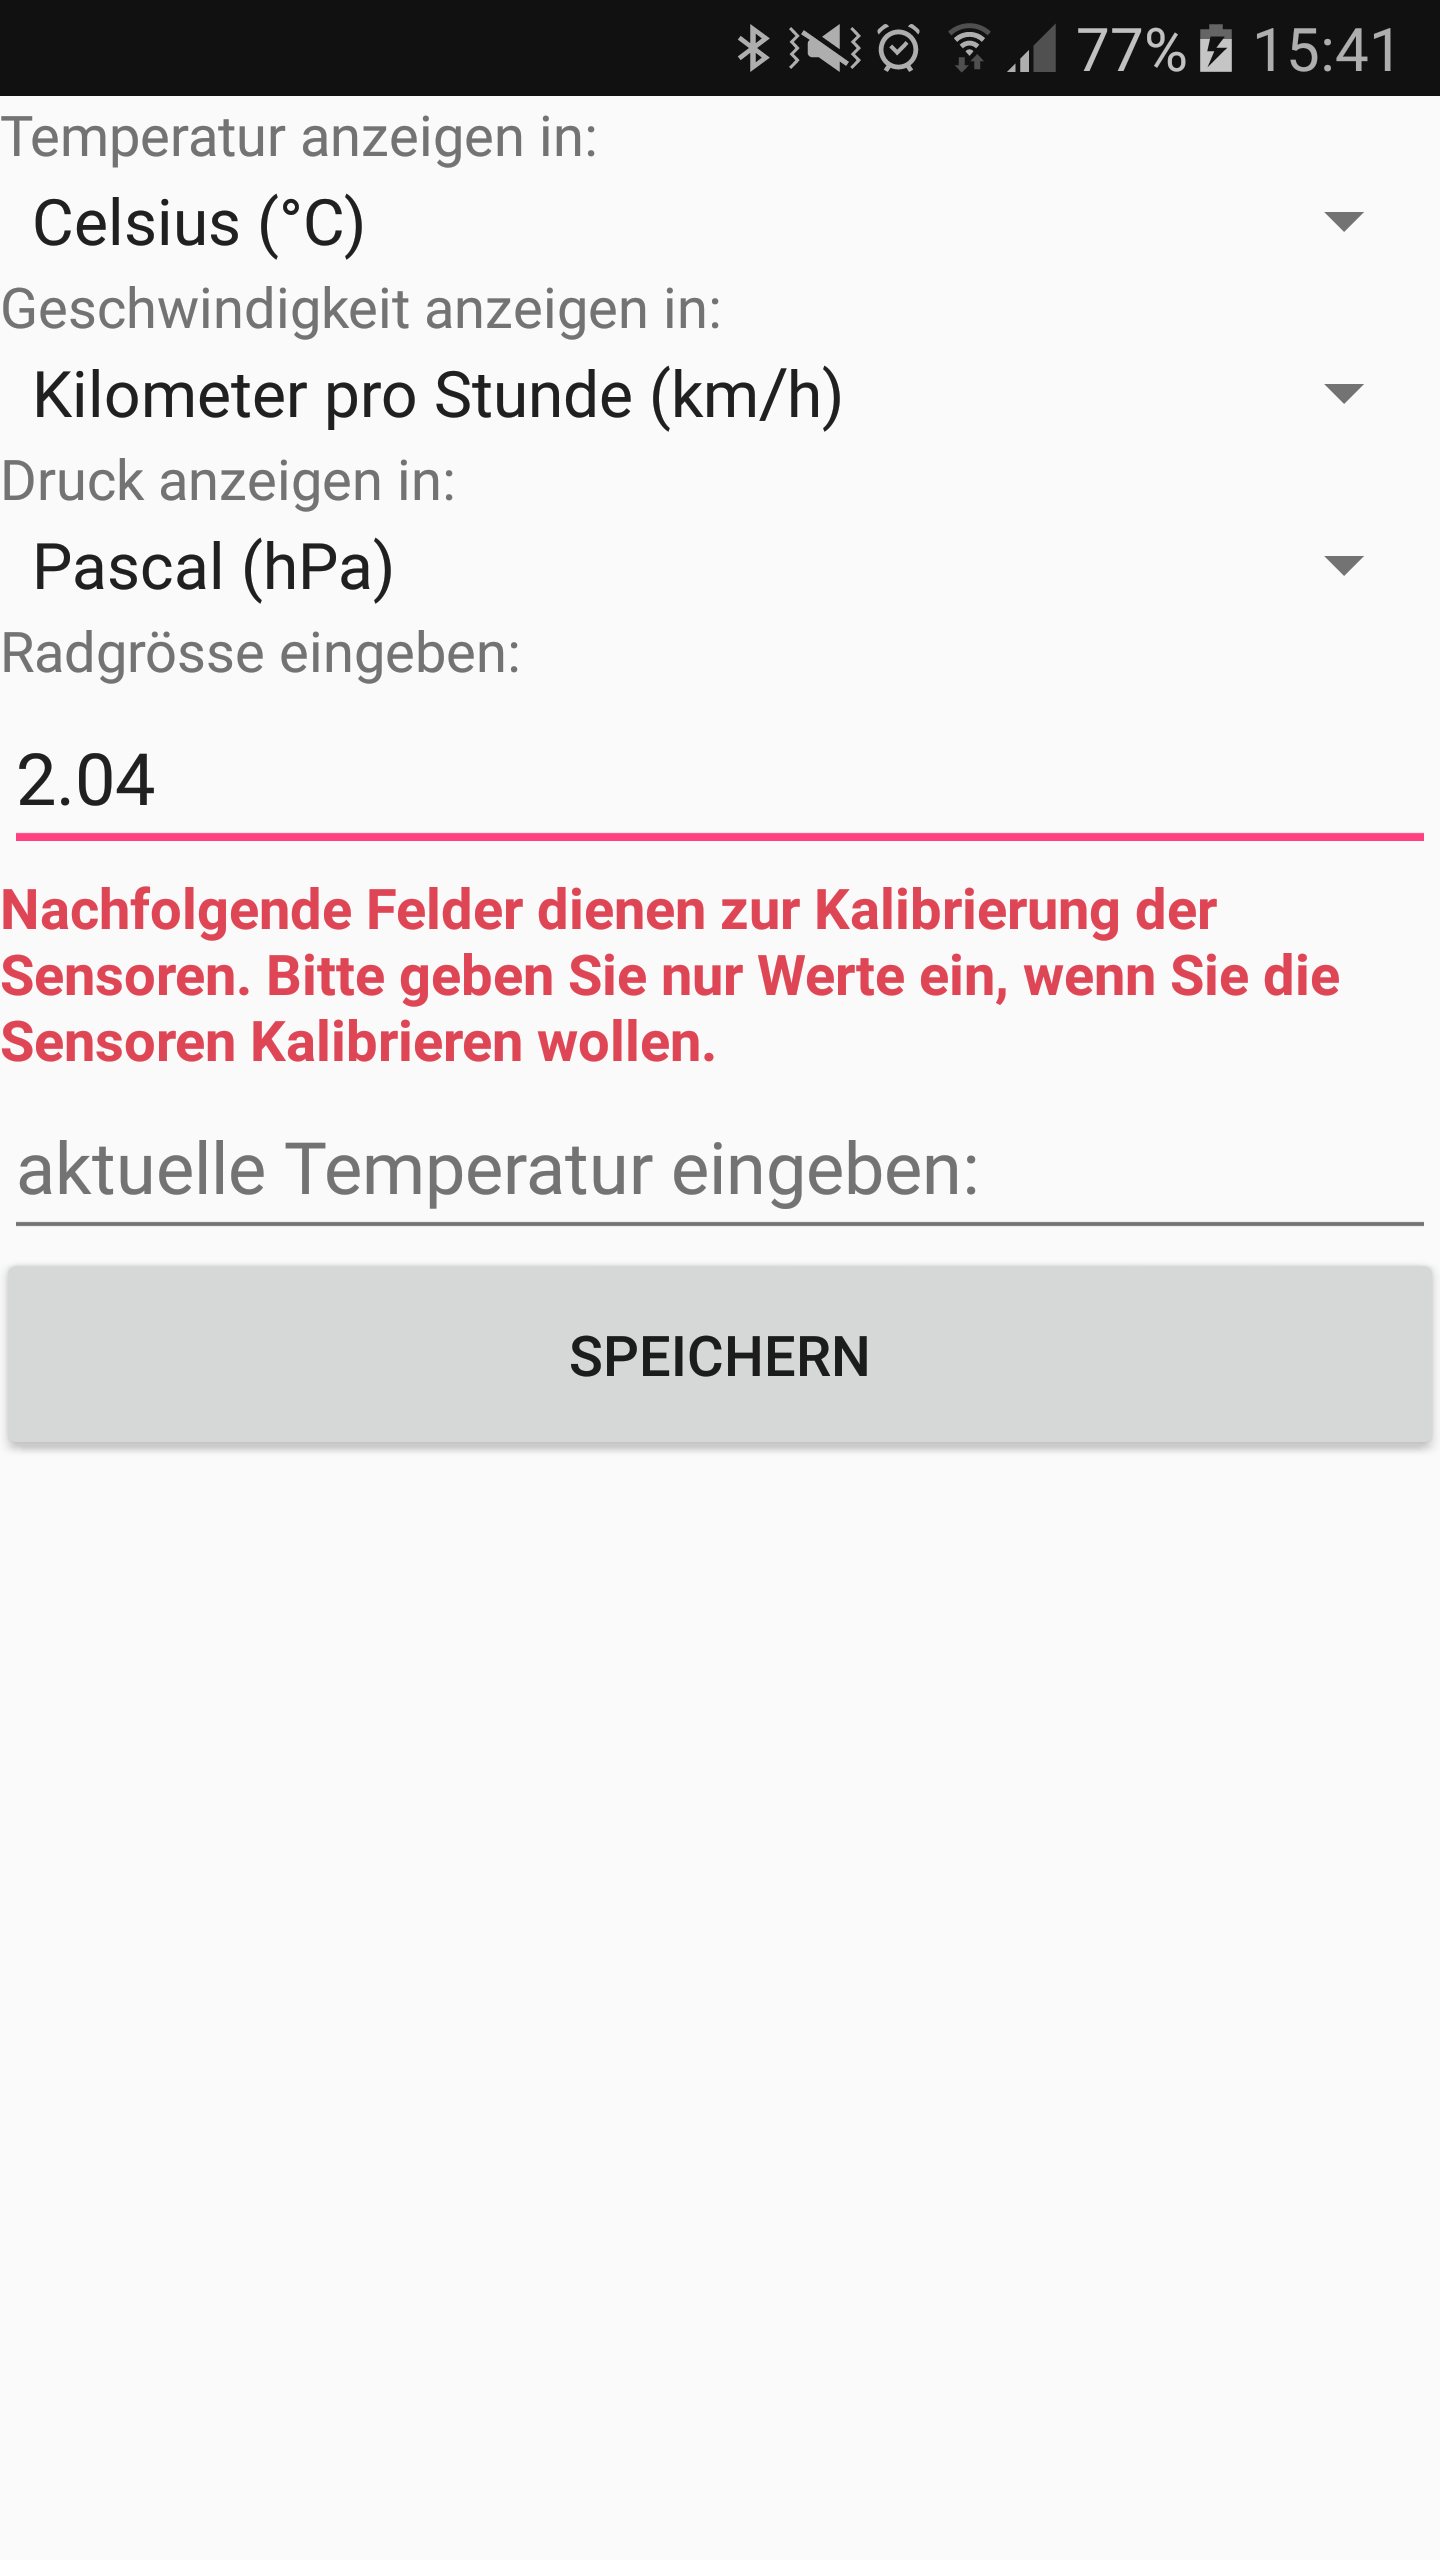
\includegraphics[width=0.5\textwidth]{4Resultate/imag/BLEEinheitenUndEinstellungenStart.png} 
    \caption{Einheiten und Einstellungen}
    \label{einheiten}
\end{figure}

Die Applikation stellt reiche Konfigurationsmöglichkeiten zur Verfügung (siehe Abbildung \ref{einheiten}. Zu jedem Sensor gehört ein Drop Down-Element, in dem die Einheiten ausgewählt werden können. Neben der Einheitenauswahl verfügt die App über die Möglichkeit, den Radumfang anzupassen und die Temperatur zu kalbrieren. 

Die Radgrösse, sprich der Radumfang, muss einstellbar sein, da die interne Geschwindigkeitsberechnung von diesem abhängt. Da die Radgrösse nicht normiert ist, konnte kein Drop Down-Element eingebaut werden. Die Zahl wird über die Tastatur in das Feld eingegeben.

Bei der Temperaturanzeige ist eine Kalibrierung eingebaut. Dies, weil alle drei Temperatursensoren auf dem Sensortag einheitlich zu hohe Werte ausgeben. Der zu hohe Temperaturwert liegt am Aufbau des Prototypen. Sensortag und Print liegen nahe aufeinander und es entsteht Wärme im Zwischenraum. Der Benutzer oder die Benutzerin kann den korrekten Wert im Kalibrationsfeld eingeben. Die nächste Temperatur, die empfangen wird, wird mit dem eingetragenen Wert verglichen und ein Offset wird eingestellt. Wird keine Kalibration eingetragen, wird die Temperatur nicht kalibriert und der Offset bleibt unverändert.

\subsubsection*{Auswählbare Einheiten}
\begin{tabbing}
    Temperatur     \quad\= Geschwindigkeit            \quad\= Druck \\[0.8ex]
    Celsius (C)    \> Kilometer pro Stunde (km/h)\> Pascal (haP)\\
    Fahrenheit (F) \> Miles per hour (mph)       \> Bar (bar)\\
    Kelvin (K)     \>                            \> Atmosph\"{a}re (atm)\\
                   \>                      \> Pound-Force per sqare inch (psi)\\
                   \>                      \> Millimeter Quecksilber (mmHG)\\
\end{tabbing} 

  
Die vorgenommenen Einstellungen werden über den Button \glqq Speichern\grqq gesichert. Danach werden die eingelesenen Sensordaten in den ausgewählten Einheiten dargestellt.

\subsection{Paketverlust}

Sensortag sendet im Advertising Mode 3 Pakete pro Sendevorgang. Gemessen wird der Paketverlust bei einer Geschwindigkeit von 20 km/h (siehe untenstehende Tabelle und \todo{Messprotokoll erwähnen}). \todo{Tabelle referenzieren}  

\subsubsection*{Paketverlust BLE-Applikation}
\begin{tabbing}
    Messperiode \quad\= Gesendete Pakete \quad\= Empfangene Pakete \quad\= Paketverlust\\[0.8ex]
    1 min  \> 38   \> 35 \> 7.9\thinspace\%  \\
    1 min  \> 37   \> 31 \> 16.2\thinspace\%  \\
    2 min  \> 75   \> 64 \> 14.7\thinspace\%  \\
    2 min  \> 77   \> 65 \> 15.6\thinspace\%  \\
    5 min  \> 193   \> 168 \> 13.0\thinspace\%  \\
    5 min  \> 190   \> 158 \> 16.8\thinspace\%  \\
    10 min  \> 345   \> 301 \> 12.8\thinspace\%  \\
    10 min  \> 349   \> 302 \> 13.5\thinspace\%  \\
\end{tabbing} 

Da der Advertising Mode keine sicher Verbindung ist, ist ein Paketverlust von rund 15\thinspace\% zu erwarten.


\subsection{Korrektheit der Daten}

Die Korrektheit der empfangenen Daten auf der Applikation wird mit einem visuellen Vergleich der Datenpakete im BLE-Sniffer von TI verglichen (siehe Abbildung \ref{sniffer}).  Die Daten im Sniffer entsprechen exakt den Daten, welche die Applikation empfängt. Der Inhalt der Daten wird somit unverfälscht übermittelt.


\todo{aktuelles Sniffer Bild} 

\begin{figure}[ht]
    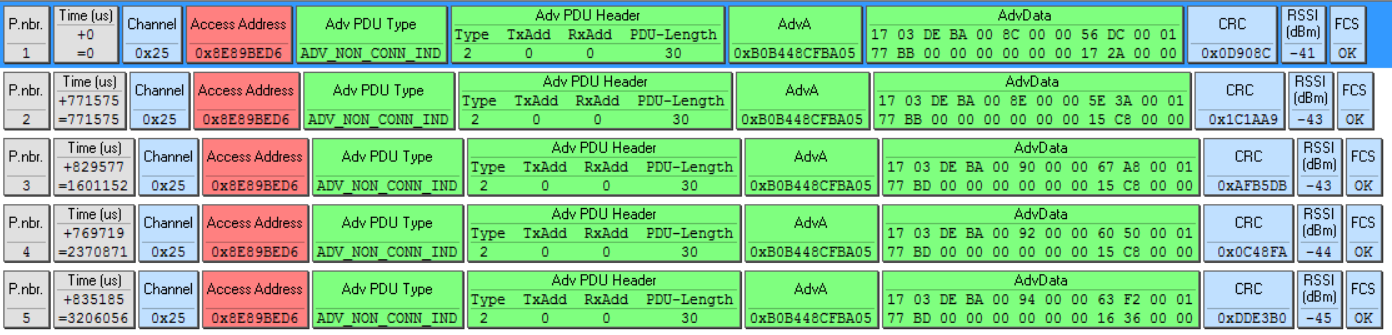
\includegraphics[width=0.5\textwidth]{4Resultate/imag/sniffer.png} 
    \caption{Snifferpaket Prototyp}
    \label{sniffer}
\end{figure}


\todo{Video zeiger (auf CD)}






